\chapter{Lecture 16 - Hydraulics II, Friction Factor and Rod-Bundle Flow}
\label{ch:ch16}
\section{Objectives}
The objectives of this lecture are:
\begin{enumerate}
\item List friction factor correlations for adiabatic and non-adiabatic flow
\item Provide a friction factor correlation to use with nuclear rod bundles.
\end{enumerate}


\section{Friction factor for Non-adiabatic and Adiabatic Flow}
\newthought{In general,} the friction factor that we use to calculate major head losses for internal flows depends not only on the geometry but whether or not the fluid is being heated, cooled, or neither.  Most experimentally-based correlations are for either flow in a circular tube or are developed in reference to flow in a circular tube; that's the geometric connection.  If a fluid is being heated or cooled (i.e. non-adiabatic) then a temperature profile is developed in the fluid at the thermal boundary layer that is different than the constant temperature profile---and consequent profile for temperature-dependent fluid properties---for adiabatic flows.  All of these have non-negligible impact on viscous energy loss and related hydraulic pressure drop.

\newthought{For adiabatic flow} in a smooth tube, we use the Karman-Nikuradse equation:
\index{Karman-Nikuradse equation}
$$\frac{1}{f}=-0.8 + 0.87 \ln{(\text{Re}\sqrt{f})}$$
Like the Colebrook equation which is used for adiabatic flow in non-smooth pipes, the Karman-Nikuradse equation requires an iterative solution that may be inconvenient.  Two frequently used approximations include the equation due to Blasius:
$$ f = 0.316 \text{Re}^{-0.25}, \ \ \ 4000 < \text{Re} < 10^5 $$ \index{Blasius equation}
or that due to McAdams:
$$f = 0.184 \text{Re}^{-0.20}, \ \ \ 10^4  <  \text{Re}  <  10^6$$ \index{McAdams equation}

Although it was mentioned in the previous lecture, for non-smooth walls we use the Colebrook equation:
$$\frac{1}{\sqrt{f}} = -2.0\log{\left(\frac{\sfrac{\epsilon}{D}}{3.7} + \frac{2.51}{\text{Re}\sqrt{f}}\right)}$$
A convenient approximation to the Colebrook equation is available using an equation due to Haaland\cite{haaland1983simple}:
$$ \frac{1}{\sqrt{f_{\text{Haaland}}}}=-1.8 \log{_{10}\left[\frac{6.9}{\text{Re}}+\left(\frac{\sfrac{\epsilon}{D}}{3.7} \right)^{1.11} \right]}$$
or another equation provided by Churchill\cite{churchill1973empirical}:
$$f_{\text{Churchill}}= \frac{8}{6.0516}\left\{\ln{\left[\frac{\sfrac{\epsilon}{D}}{3.7}+\left(\frac{7}{\text{Re}} \right)^{0.9} \right]} \right\}^{-2}$$
\marginnote[-0.25cm]{\textbf{Note: }If you have multiple approximations, it does not hurt to try both! Pick whichever one is the most accurate or conservative in accordance with your willingness to accept risk.}
\index{hydraulic diameter}
In all cases above, the Reynolds number is based on the diameter of the circular channel.  In cases where the channel is not circular and where you would like to use the correlations anyway, you should calculate the Reynolds number relative to the \emph{hydraulic diameter}.\marginnote[0.25cm]{\textbf{hydraulic diameter} is computed as: $D_h = \frac{4 A_{\text{flow}}}{P_{\text{wetted}}}$ where $A_{\text{flow}}$ is the cross sectional flow area and $P_{\text{wetted}}$ is the wetted perimeter.  } 

\section{Diabatic Flow}
\newthought{If heat is being added} or removed from the fluid then there is a temperature gradient within the fluid.  Temperature-dependent properties like density and viscosity vary in the direction along which heat is moving.  For example, when heat is transferred from primary to secondary coolant in the steam generator of PWR, primary coolant next to the U-tube wall is at a lower temperature than coolant near the center of the tube.  Consequently the viscosity of the fluid - which for liquids tends to vary inversely with temperature - will be higher.  This changes the friction factor and that change should be taken into account.

For this class we will use the correlation due to Petukhov\cite{petukhov1970heat}. This correlation includes a basic friction factor: \index{Petukhov correlation}

$$ f_{T_{b}}= \left(1.82 \log{_{10}\text{Re}_{D}}-1.64  \right)^{-2}, \ \ \ 3000 < \text{Re} < 5\times 10^6$$
where $\text{Re}_{D}$ is the Reynolds number based on tube diameter (or hydraulic diameter) with fluid properties evaluated at their bulk average (i.e. not along the tube wall) temperature.\marginnote[-0.5cm]{\textbf{Note:} The term $T_{b}$, as part of $f_{\text{T}_b}$, should be read as ``...at bulk temperature.''} The final friction factor is then found using the following formula depending on whether the fluid is a gas or liquid and whether the fluid is being heated or cooled.
For liquids:
$$\frac{f}{f_{T_b}}=g\left(\frac{\mu_b}{\mu_w} \right), \ \ \ 0.5 \le \sfrac{\mu_b}{\mu_w} \le 3$$
where $\mu_b$ is the bulk viscosity and $\mu_w$ is the viscosity of the fluid adjacent to the wall.  The function $g(\sfrac{\mu_b}{\mu_w})$ is different for heating and cooling. 
For heating:
$$g(\sfrac{\mu_b}{\mu_w})=\frac{1}{6}\left(7 - \frac{\mu_b}{\mu_w} \right)$$
For cooling:
$$g(\sfrac{\mu_b}{\mu_w})=\left(\frac{\mu_b}{\mu_w} \right)^{-0.24}$$
For gasses, the relation is:
$$\frac{f}{f_{T_b}}=\left(\frac{T_b}{T_w} \right)^{0.23}, \ \ \ 0.14 \le \sfrac{T_b}{T_w} \le 3.3 $$
This relation is used for both heating and cooling.


\section{Pressure Drop in Rod Bundles}

\newthought{The friction factor} for fluid flow in a rod bundle depends on a number of factors.  The factors that we will take into account with the correlation we will use include:

\begin{marginfigure}
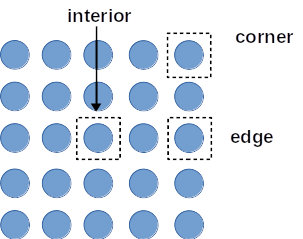
\includegraphics{assy_position.png}
\caption{Rod assembly channel positions for a rectangular bundle.}
\label{fig:assy_position}
\end{marginfigure}

\begin{itemize}
\item whether the flow is laminar or turbulent;
\item whether the rod bundle is a rectangular or hexagonal array;
\item channel position within a fuel assembly; and 
\item how closely packed the rod bundles are
\end{itemize}
the last term we will parameterize by the pitch-to-diameter ratio of the rod bundle.\marginnote[-1.20cm]{\textbf{Rod pitch} is the distance between the center-line of adjacent rods.  The \textbf{pitch-to-diameter ratio} $\left(\sfrac{P}{D} \right)$non-dimensionalizes this distance.  The minimum possible value of $\sfrac{P}{D}$ is 1 when the rods are touching.  Typical $\sfrac{P}{D}$ for a LWR is approximately 1.4.}  The channel position may correspond to an interior, edge, or corner channel as illustrated by Figure \ref{fig:assy_position}.  

All of these factors are included in the Cheng-Todreas correlation\cite{cheng1986hydrodynamic} that we will use.  The general form of the correlation is given by:
$$f = \frac{C}{\text{Re}^n}$$
The numerator $C$ is a quadratic function of pitch-to-diameter ratio:
$$C = a + b_1\left(\frac{P}{D}-1\right)+b_2\left(\frac{P}{D}-1\right)^2$$
in which the coefficients depend on whether the flow is laminar or turbulent, whether the rod bundle is rectangular or hexagonal, whether the subchannel is an edge, corner,or interior channel and the pitch-to-diameter ratio.  Coefficient values for rectangular channels are provided in Table \ref{tab:cheng-todreas-sq}; values for hexagonal channels are provided in Table \ref{tab:cheng-todreas-hex}.
\begin{table}
\begin{tabular}{c c c c c c c}
\toprule
  & \multicolumn{3}{c}{$1.0 \le P/D < 1.1$} & \multicolumn{3}{c}{$1.1 \le P/D \le 1.5$} \\
  \cmidrule(lr){2-4} \cmidrule(lr){5-7}
 & $a$ & $b_1$ & $b_2$ & $a$ & $b_1$ & $b_2$ \\
  & \multicolumn{6}{c}{\textbf{Laminar Flow}} \\
interior  & 26.37 & 374.2 & -493.9 & 35.55 & 263.7 & -190.2 \\
edge      & 26.18 & 554.5 & -1480 & 44.40 & 256.7 & -267.6 \\
corner    & 28.62 & 715.9 & -2807 & 58.83 & 160.7 & -203.5 \\
& \multicolumn{6}{c}{\textbf{Turbulent Flow}} \\
interior & 0.09423 & 0.5806 & -1.239 & 0.1339 & 0.09059 & -0.09926 \\
edge     & 0.09377 & 0.8732 & -3.341 & 0.1430 & 0.04199 & -0.04428 \\
corner   & 0.09755 & 1.127 & -6.304 & 0.1452 & 0.02681 & -0.03411 \\
\bottomrule
\end{tabular}
\caption{Coefficients for the Cheng-Todreas correlation for a square array.}
\label{tab:cheng-todreas-sq}
\end{table}
\begin{table}
\begin{tabular}{c c c c c c c}
\toprule
  & \multicolumn{3}{c}{$1.0 \le P/D < 1.1$} & \multicolumn{3}{c}{$1.1 \le P/D \le 1.5$} \\
  \cmidrule(lr){2-4} \cmidrule(lr){5-7}
 & $a$ & $b_1$ & $b_2$ & $a$ & $b_1$ & $b_2$ \\
  & \multicolumn{6}{c}{\textbf{Laminar Flow}} \\
interior  & 26.00 & 888.2 & -3334 & 62.97 & 216.9 & -190.2 \\
edge      & 26.18 & 554.5 & -1480 & 44.40 & 256.7 & -267.6 \\
corner    & 28.98 & 1636 & -10050 & 87.26 & 38.59 & -55.12 \\
& \multicolumn{6}{c}{\textbf{Turbulent Flow}} \\
interior & 0.09378 & 1.398 & -8.664 & 0.1458 & 0.03632 & -0.03333 \\
edge     & 0.09377 & 0.8732 & -3.341 & 0.1430 & 0.04199 & -0.04428 \\
corner   & 0.1004 & 1.625 & -11.85 & 0.1499 & 0.006706 & -0.009567 \\
\bottomrule
\end{tabular}
\caption{Coefficients for the Cheng-Todreas correlation for a hexagonal array.}
\label{tab:cheng-todreas-hex}
\end{table}
For laminar flow, $n=1$.  For turbulent flow, $n=0.18$.

In all cases, the Reynolds number is calculated relative to the hydraulic diameter.  Calculation of flow area $(\text{A}_{\text{flow}})$ and wetted perimeter $(\text{P}_{\text{wetted}})$ for rectangular and hexagonal arrays are as shown in Figure \ref{fig:equiv-a}.
\begin{marginfigure}
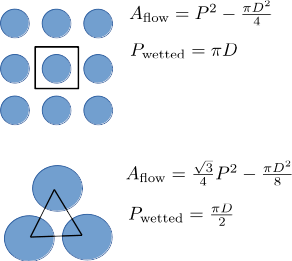
\includegraphics{equiv_annulus.png}
\caption{Calculation of flow area and wetted perimeter for flow channel within a rod bundle.}
\label{fig:equiv-a}
\end{marginfigure}  

\section{Parting Note}
This lecture provides a simplified but reasonably complete presentation of what I judge to be the most important hydraulic correlations for single-phase viscous fluid flow.  One important phenomena that I have not treated at all is for the friction factor near the entrance of a circular tube or fuel assembly.  This region of ``developing flow'' is where the fluid adjusts to the presence of channel walls where before there were none.  As you might expect, there is considerable ``action'' in the fluid flow field at such a point.  For hydraulic analysis this means that, near the entrance of a channel you can expect the \emph{actual} friction factor to be \underline{higher} than what we have calculated for the fully-developed flow.  While we will consider this detail to be outside the scope of this class, state-of-the-art hydraulic analysis codes take this effect into account.

